% Generated by ArticleSignalDiagrams. Opaque vector fills only.
\documentclass[10pt,tikz,border=5pt]{standalone}
\usepackage{lmodern}
\usetikzlibrary{fit}
\begin{document}
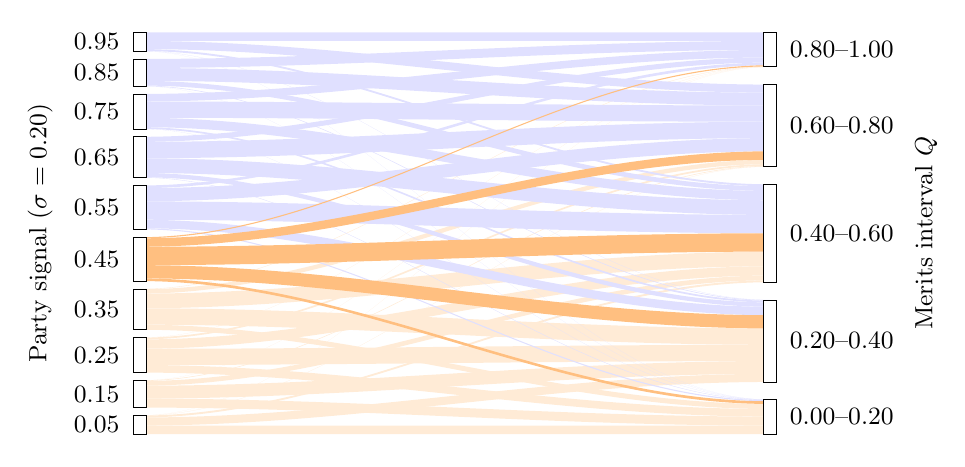
\begin{tikzpicture}[x=1cm,y=1cm,font=\small]\path[fill=orange!16!white,draw=none] (3.3,-5.1) .. controls (6,-5.1) and (8.6,-5.1) .. (11.3,-5.1) -- (11.3,-4.992409) .. controls (8.6,-4.992409) and (6,-4.992409) .. (3.3,-4.992409) -- cycle;
\path[fill=orange!16!white,draw=none] (3.3,-4.992409) .. controls (6,-4.992409) and (8.6,-4.4382) .. (11.3,-4.4382) -- (11.3,-4.335559) .. controls (8.6,-4.335559) and (6,-4.889769) .. (3.3,-4.889769) -- cycle;
\path[fill=orange!16!white,draw=none] (3.3,-4.889769) .. controls (6,-4.889769) and (8.6,-3.1716) .. (11.3,-3.1716) -- (11.3,-3.147371) .. controls (8.6,-3.147371) and (6,-4.86554) .. (3.3,-4.86554) -- cycle;
\path[fill=orange!16!white,draw=none] (3.3,-4.86554) .. controls (6,-4.86554) and (8.6,-1.7034) .. (11.3,-1.7034) -- (11.3,-1.701543) .. controls (8.6,-1.701543) and (6,-4.863682) .. (3.3,-4.863682) -- cycle;
\path[fill=orange!16!white,draw=none] (3.3,-4.863682) .. controls (6,-4.863682) and (8.6,-0.4368) .. (11.3,-0.4368) -- (11.3,-0.436758) .. controls (8.6,-0.436758) and (6,-4.863641) .. (3.3,-4.863641) -- cycle;
\path[fill=orange!16!white,draw=none] (3.3,-4.763641) .. controls (6,-4.763641) and (8.6,-4.992409) .. (11.3,-4.992409) -- (11.3,-4.878233) .. controls (8.6,-4.878233) and (6,-4.649464) .. (3.3,-4.649464) -- cycle;
\path[fill=orange!16!white,draw=none] (3.3,-4.649464) .. controls (6,-4.649464) and (8.6,-4.335559) .. (11.3,-4.335559) -- (11.3,-4.172723) .. controls (8.6,-4.172723) and (6,-4.486628) .. (3.3,-4.486628) -- cycle;
\path[fill=orange!16!white,draw=none] (3.3,-4.486628) .. controls (6,-4.486628) and (8.6,-3.147371) .. (11.3,-3.147371) -- (11.3,-3.087353) .. controls (8.6,-3.087353) and (6,-4.426609) .. (3.3,-4.426609) -- cycle;
\path[fill=orange!16!white,draw=none] (3.3,-4.426609) .. controls (6,-4.426609) and (8.6,-1.701543) .. (11.3,-1.701543) -- (11.3,-1.694298) .. controls (8.6,-1.694298) and (6,-4.419365) .. (3.3,-4.419365) -- cycle;
\path[fill=orange!16!white,draw=none] (3.3,-4.419365) .. controls (6,-4.419365) and (8.6,-0.436758) .. (11.3,-0.436758) -- (11.3,-0.436502) .. controls (8.6,-0.436502) and (6,-4.419108) .. (3.3,-4.419108) -- cycle;
\path[fill=orange!16!white,draw=none] (3.3,-4.319108) .. controls (6,-4.319108) and (8.6,-4.878233) .. (11.3,-4.878233) -- (11.3,-4.782048) .. controls (8.6,-4.782048) and (6,-4.222923) .. (3.3,-4.222923) -- cycle;
\path[fill=orange!16!white,draw=none] (3.3,-4.222923) .. controls (6,-4.222923) and (8.6,-4.172723) .. (11.3,-4.172723) -- (11.3,-3.96664) .. controls (8.6,-3.96664) and (6,-4.01684) .. (3.3,-4.01684) -- cycle;
\path[fill=orange!16!white,draw=none] (3.3,-4.01684) .. controls (6,-4.01684) and (8.6,-3.087353) .. (11.3,-3.087353) -- (11.3,-2.969009) .. controls (8.6,-2.969009) and (6,-3.898497) .. (3.3,-3.898497) -- cycle;
\path[fill=orange!16!white,draw=none] (3.3,-3.898497) .. controls (6,-3.898497) and (8.6,-1.694298) .. (11.3,-1.694298) -- (11.3,-1.671884) .. controls (8.6,-1.671884) and (6,-3.876083) .. (3.3,-3.876083) -- cycle;
\path[fill=orange!16!white,draw=none] (3.3,-3.876083) .. controls (6,-3.876083) and (8.6,-0.436502) .. (11.3,-0.436502) -- (11.3,-0.435263) .. controls (8.6,-0.435263) and (6,-3.874843) .. (3.3,-3.874843) -- cycle;
\path[fill=orange!16!white,draw=none] (3.3,-3.774843) .. controls (6,-3.774843) and (8.6,-4.782048) .. (11.3,-4.782048) -- (11.3,-4.717775) .. controls (8.6,-4.717775) and (6,-3.71057) .. (3.3,-3.71057) -- cycle;
\path[fill=orange!16!white,draw=none] (3.3,-3.71057) .. controls (6,-3.71057) and (8.6,-3.96664) .. (11.3,-3.96664) -- (11.3,-3.758529) .. controls (8.6,-3.758529) and (6,-3.50246) .. (3.3,-3.50246) -- cycle;
\path[fill=orange!16!white,draw=none] (3.3,-3.50246) .. controls (6,-3.50246) and (8.6,-2.969009) .. (11.3,-2.969009) -- (11.3,-2.783052) .. controls (8.6,-2.783052) and (6,-3.316503) .. (3.3,-3.316503) -- cycle;
\path[fill=orange!16!white,draw=none] (3.3,-3.316503) .. controls (6,-3.316503) and (8.6,-1.671884) .. (11.3,-1.671884) -- (11.3,-1.616802) .. controls (8.6,-1.616802) and (6,-3.261421) .. (3.3,-3.261421) -- cycle;
\path[fill=orange!16!white,draw=none] (3.3,-3.261421) .. controls (6,-3.261421) and (8.6,-0.435263) .. (11.3,-0.435263) -- (11.3,-0.430531) .. controls (8.6,-0.430531) and (6,-3.256689) .. (3.3,-3.256689) -- cycle;
\path[fill=blue!12!white,draw=none] (3.3,-2.5) .. controls (6,-2.5) and (8.6,-4.683738) .. (11.3,-4.683738) -- (11.3,-4.669469) .. controls (8.6,-4.669469) and (6,-2.48573) .. (3.3,-2.48573) -- cycle;
\path[fill=blue!12!white,draw=none] (3.3,-2.48573) .. controls (6,-2.48573) and (8.6,-3.590876) .. (11.3,-3.590876) -- (11.3,-3.483198) .. controls (8.6,-3.483198) and (6,-2.378052) .. (3.3,-2.378052) -- cycle;
\path[fill=blue!12!white,draw=none] (3.3,-2.378052) .. controls (6,-2.378052) and (8.6,-2.55) .. (11.3,-2.55) -- (11.3,-2.316948) .. controls (8.6,-2.316948) and (6,-2.145) .. (3.3,-2.145) -- cycle;
\path[fill=blue!12!white,draw=none] (3.3,-2.145) .. controls (6,-2.145) and (8.6,-1.509124) .. (11.3,-1.509124) -- (11.3,-1.341471) .. controls (8.6,-1.341471) and (6,-1.977347) .. (3.3,-1.977347) -- cycle;
\path[fill=blue!12!white,draw=none] (3.3,-1.977347) .. controls (6,-1.977347) and (8.6,-0.416262) .. (11.3,-0.416262) -- (11.3,-0.382225) .. controls (8.6,-0.382225) and (6,-1.943311) .. (3.3,-1.943311) -- cycle;
\path[fill=blue!12!white,draw=none] (3.3,-1.843311) .. controls (6,-1.843311) and (8.6,-4.669469) .. (11.3,-4.669469) -- (11.3,-4.664737) .. controls (8.6,-4.664737) and (6,-1.838579) .. (3.3,-1.838579) -- cycle;
\path[fill=blue!12!white,draw=none] (3.3,-1.838579) .. controls (6,-1.838579) and (8.6,-3.483198) .. (11.3,-3.483198) -- (11.3,-3.428116) .. controls (8.6,-3.428116) and (6,-1.783497) .. (3.3,-1.783497) -- cycle;
\path[fill=blue!12!white,draw=none] (3.3,-1.783497) .. controls (6,-1.783497) and (8.6,-2.316948) .. (11.3,-2.316948) -- (11.3,-2.130991) .. controls (8.6,-2.130991) and (6,-1.59754) .. (3.3,-1.59754) -- cycle;
\path[fill=blue!12!white,draw=none] (3.3,-1.59754) .. controls (6,-1.59754) and (8.6,-1.341471) .. (11.3,-1.341471) -- (11.3,-1.13336) .. controls (8.6,-1.13336) and (6,-1.38943) .. (3.3,-1.38943) -- cycle;
\path[fill=blue!12!white,draw=none] (3.3,-1.38943) .. controls (6,-1.38943) and (8.6,-0.382225) .. (11.3,-0.382225) -- (11.3,-0.317952) .. controls (8.6,-0.317952) and (6,-1.325157) .. (3.3,-1.325157) -- cycle;
\path[fill=blue!12!white,draw=none] (3.3,-1.225157) .. controls (6,-1.225157) and (8.6,-4.664737) .. (11.3,-4.664737) -- (11.3,-4.663498) .. controls (8.6,-4.663498) and (6,-1.223917) .. (3.3,-1.223917) -- cycle;
\path[fill=blue!12!white,draw=none] (3.3,-1.223917) .. controls (6,-1.223917) and (8.6,-3.428116) .. (11.3,-3.428116) -- (11.3,-3.405702) .. controls (8.6,-3.405702) and (6,-1.201503) .. (3.3,-1.201503) -- cycle;
\path[fill=blue!12!white,draw=none] (3.3,-1.201503) .. controls (6,-1.201503) and (8.6,-2.130991) .. (11.3,-2.130991) -- (11.3,-2.012647) .. controls (8.6,-2.012647) and (6,-1.08316) .. (3.3,-1.08316) -- cycle;
\path[fill=blue!12!white,draw=none] (3.3,-1.08316) .. controls (6,-1.08316) and (8.6,-1.13336) .. (11.3,-1.13336) -- (11.3,-0.927277) .. controls (8.6,-0.927277) and (6,-0.877077) .. (3.3,-0.877077) -- cycle;
\path[fill=blue!12!white,draw=none] (3.3,-0.877077) .. controls (6,-0.877077) and (8.6,-0.317952) .. (11.3,-0.317952) -- (11.3,-0.221767) .. controls (8.6,-0.221767) and (6,-0.780892) .. (3.3,-0.780892) -- cycle;
\path[fill=blue!12!white,draw=none] (3.3,-0.680892) .. controls (6,-0.680892) and (8.6,-4.663498) .. (11.3,-4.663498) -- (11.3,-4.663242) .. controls (8.6,-4.663242) and (6,-0.680635) .. (3.3,-0.680635) -- cycle;
\path[fill=blue!12!white,draw=none] (3.3,-0.680635) .. controls (6,-0.680635) and (8.6,-3.405702) .. (11.3,-3.405702) -- (11.3,-3.398457) .. controls (8.6,-3.398457) and (6,-0.673391) .. (3.3,-0.673391) -- cycle;
\path[fill=blue!12!white,draw=none] (3.3,-0.673391) .. controls (6,-0.673391) and (8.6,-2.012647) .. (11.3,-2.012647) -- (11.3,-1.952629) .. controls (8.6,-1.952629) and (6,-0.613372) .. (3.3,-0.613372) -- cycle;
\path[fill=blue!12!white,draw=none] (3.3,-0.613372) .. controls (6,-0.613372) and (8.6,-0.927277) .. (11.3,-0.927277) -- (11.3,-0.764441) .. controls (8.6,-0.764441) and (6,-0.450536) .. (3.3,-0.450536) -- cycle;
\path[fill=blue!12!white,draw=none] (3.3,-0.450536) .. controls (6,-0.450536) and (8.6,-0.221767) .. (11.3,-0.221767) -- (11.3,-0.107591) .. controls (8.6,-0.107591) and (6,-0.336359) .. (3.3,-0.336359) -- cycle;
\path[fill=blue!12!white,draw=none] (3.3,-0.236359) .. controls (6,-0.236359) and (8.6,-4.663242) .. (11.3,-4.663242) -- (11.3,-4.6632) .. controls (8.6,-4.6632) and (6,-0.236318) .. (3.3,-0.236318) -- cycle;
\path[fill=blue!12!white,draw=none] (3.3,-0.236318) .. controls (6,-0.236318) and (8.6,-3.398457) .. (11.3,-3.398457) -- (11.3,-3.3966) .. controls (8.6,-3.3966) and (6,-0.23446) .. (3.3,-0.23446) -- cycle;
\path[fill=blue!12!white,draw=none] (3.3,-0.23446) .. controls (6,-0.23446) and (8.6,-1.952629) .. (11.3,-1.952629) -- (11.3,-1.9284) .. controls (8.6,-1.9284) and (6,-0.210231) .. (3.3,-0.210231) -- cycle;
\path[fill=blue!12!white,draw=none] (3.3,-0.210231) .. controls (6,-0.210231) and (8.6,-0.764441) .. (11.3,-0.764441) -- (11.3,-0.6618) .. controls (8.6,-0.6618) and (6,-0.107591) .. (3.3,-0.107591) -- cycle;
\path[fill=blue!12!white,draw=none] (3.3,-0.107591) .. controls (6,-0.107591) and (8.6,-0.107591) .. (11.3,-0.107591) -- (11.3,-0) .. controls (8.6,-0) and (6,0) .. (3.3,0) -- cycle;
\path[fill=orange!50!white,draw=none] (3.3,-3.156689) .. controls (6,-3.156689) and (8.6,-4.717775) .. (11.3,-4.717775) -- (11.3,-4.683738) .. controls (8.6,-4.683738) and (6,-3.122653) .. (3.3,-3.122653) -- cycle;
\path[fill=orange!50!white,draw=none] (3.3,-3.122653) .. controls (6,-3.122653) and (8.6,-3.758529) .. (11.3,-3.758529) -- (11.3,-3.590876) .. controls (8.6,-3.590876) and (6,-2.955) .. (3.3,-2.955) -- cycle;
\path[fill=orange!50!white,draw=none] (3.3,-2.955) .. controls (6,-2.955) and (8.6,-2.783052) .. (11.3,-2.783052) -- (11.3,-2.55) .. controls (8.6,-2.55) and (6,-2.721948) .. (3.3,-2.721948) -- cycle;
\path[fill=orange!50!white,draw=none] (3.3,-2.721948) .. controls (6,-2.721948) and (8.6,-1.616802) .. (11.3,-1.616802) -- (11.3,-1.509124) .. controls (8.6,-1.509124) and (6,-2.61427) .. (3.3,-2.61427) -- cycle;
\path[fill=orange!50!white,draw=none] (3.3,-2.61427) .. controls (6,-2.61427) and (8.6,-0.430531) .. (11.3,-0.430531) -- (11.3,-0.416262) .. controls (8.6,-0.416262) and (6,-2.6) .. (3.3,-2.6) -- cycle;
\coordinate (axis-midline-0) at (0,-2.55);
\path[fill=white,draw=black,line width=0.3pt] (3.22,-5.1) rectangle (3.38,-4.863641);
\node[anchor=east,fill=white,inner sep=2pt] (bucket-0-0-0) at (3.12,-4.98182) {0.05};
\path[fill=white,draw=black,line width=0.3pt] (3.22,-4.763641) rectangle (3.38,-4.419108);
\node[anchor=east,fill=white,inner sep=2pt] (bucket-0-0-1) at (3.12,-4.591375) {0.15};
\path[fill=white,draw=black,line width=0.3pt] (3.22,-4.319108) rectangle (3.38,-3.874843);
\node[anchor=east,fill=white,inner sep=2pt] (bucket-0-0-2) at (3.12,-4.096976) {0.25};
\path[fill=white,draw=black,line width=0.3pt] (3.22,-3.774843) rectangle (3.38,-3.256689);
\node[anchor=east,fill=white,inner sep=2pt] (bucket-0-0-3) at (3.12,-3.515766) {0.35};
\path[fill=white,draw=black,line width=0.3pt] (3.22,-3.156689) rectangle (3.38,-2.6);
\node[anchor=east,fill=white,inner sep=2pt] (bucket-0-0-4) at (3.12,-2.878345) {0.45};
\path[fill=white,draw=black,line width=0.3pt] (3.22,-2.5) rectangle (3.38,-1.943311);
\node[anchor=east,fill=white,inner sep=2pt] (bucket-0-0-5) at (3.12,-2.221655) {0.55};
\path[fill=white,draw=black,line width=0.3pt] (3.22,-1.843311) rectangle (3.38,-1.325157);
\node[anchor=east,fill=white,inner sep=2pt] (bucket-0-0-6) at (3.12,-1.584234) {0.65};
\path[fill=white,draw=black,line width=0.3pt] (3.22,-1.225157) rectangle (3.38,-0.780892);
\node[anchor=east,fill=white,inner sep=2pt] (bucket-0-0-7) at (3.12,-1.003024) {0.75};
\path[fill=white,draw=black,line width=0.3pt] (3.22,-0.680892) rectangle (3.38,-0.336359);
\node[anchor=east,fill=white,inner sep=2pt] (bucket-0-0-8) at (3.12,-0.508625) {0.85};
\path[fill=white,draw=black,line width=0.3pt] (3.22,-0.236359) rectangle (3.38,0);
\node[anchor=east,fill=white,inner sep=2pt] (bucket-0-0-9) at (3.12,-0.11818) {0.95};
\node[fit=(bucket-0-0-0) (bucket-0-0-1) (bucket-0-0-2) (bucket-0-0-3) (bucket-0-0-4) (bucket-0-0-5) (bucket-0-0-6) (bucket-0-0-7) (bucket-0-0-8) (bucket-0-0-9),inner sep=0pt] (source-labels-0) {};
\coordinate (axis-title-0-0) at (source-labels-0.west |- axis-midline-0);
\node[rotate=90,anchor=south,inner sep=0pt] at ([xshift=-0.18cm]axis-title-0-0) {Party signal ($\sigma=0.20$)};
\path[fill=white,draw=black,line width=0.3pt] (11.22,-5.1) rectangle (11.38,-4.6632);
\node[anchor=west,fill=white,inner sep=2pt] (bucket-0-1-0) at (11.48,-4.8816) {0.00--0.20};
\path[fill=white,draw=black,line width=0.3pt] (11.22,-4.4382) rectangle (11.38,-3.3966);
\node[anchor=west,fill=white,inner sep=2pt] (bucket-0-1-1) at (11.48,-3.9174) {0.20--0.40};
\path[fill=white,draw=black,line width=0.3pt] (11.22,-3.1716) rectangle (11.38,-1.9284);
\node[anchor=west,fill=white,inner sep=2pt] (bucket-0-1-2) at (11.48,-2.55) {0.40--0.60};
\path[fill=white,draw=black,line width=0.3pt] (11.22,-1.7034) rectangle (11.38,-0.6618);
\node[anchor=west,fill=white,inner sep=2pt] (bucket-0-1-3) at (11.48,-1.1826) {0.60--0.80};
\path[fill=white,draw=black,line width=0.3pt] (11.22,-0.4368) rectangle (11.38,-0);
\node[anchor=west,fill=white,inner sep=2pt] (bucket-0-1-4) at (11.48,-0.2184) {0.80--1.00};
\node[fit=(bucket-0-1-0) (bucket-0-1-1) (bucket-0-1-2) (bucket-0-1-3) (bucket-0-1-4),inner sep=0pt] (destination-labels-0) {};
\coordinate (axis-title-0-1) at (destination-labels-0.east |- axis-midline-0);
\node[rotate=90,anchor=north,inner sep=0pt] at ([xshift=0.18cm]axis-title-0-1) {Merits interval $Q$};
\end{tikzpicture}
\end{document}

